% !TEX root = main.tex

\section{曲线积分与曲面积分}
\subsection{第一型曲线及曲面积分}
\begin{definition}[第一型曲线积分]
设$L$为空间可求长的曲线段,$f(x,y,z)$定义在$L$上,$L$的两端点为$A,B$,依次用分点$A=A_0,A_1,\ldots,A_n=B$将$L$分为$n$小段,每小段的弧长记为$\Delta s_i$,不妨将第$i$段小弧也记为$\Delta s_i$,任取$(\xi_i,\eta_i,\zeta_i)\in\Delta s_i$,作和式
\[\sum_{i=1}^n f(\xi_i,\eta_i,\zeta_i)\Delta s_i\]
若当$\lambda=\max_{1\leq i\leq n}\{\Delta s_i\}\to 0$时上述和式极限存在,则称此极限值为$f(x,y,z)$在曲线$L$上的第一型曲线积分,记为
\[\int_Lf(x,y,z)\diff s=\lim_{\lambda\to 0}\sum_{i=1}^nf(\xi_i,\eta_i,\zeta_i)\Delta s_i\]
若$L$为光滑曲线
\[x=x(t),y=y(t),z=z(t),\alpha\leq t\leq\beta\]
$f(x,y,z)$在$L$上连续,则$f(x,y,z)$在$L$上的第一型曲线积分存在,有
\[\int_Lf(x,y,z)\diff s=\intabu{\alpha}{\beta}{f(x(t),y(t),z(t))\sqrt{{x'}^2(t)+{y'}^2(t)+{z'}^2(t)}}{t}\]
\end{definition}
由于第一型曲线积分是无向的(上限一定大于下限),故
\[\int_{\wideparen{AB}}f(x,y,z)\diff s=\int_{\wideparen{BA}}f(x,y,z)\diff s\]
\begin{definition}[第一型曲面积分]
设$S$是空间光滑曲面$z=z(x,y),(x,y)\in D$,$f(x,y,z)$是定义在$S$上的函数,对于$D$的任意分法$\Delta\sigma_i$,相应地得到$S$的分法$\Delta S_i$,任取$(\xi_i,\eta_i,\zeta_i)\in\Delta S_i$,记$\lambda=\max_{1\leq i\leq n}\{d(\Delta\sigma_i)\}$,则第一型曲面积分记为
\[\iint_S f(x,y,z)\diff S=\lim_{\lambda\to 0}\sum_{i=1}^n f(\xi_i,\eta_i,\zeta_i)\Delta S_i\]
若$D$为有界闭区域,$f(x,y,z)$在$S$上连续,则$f(x,y,z)$在曲面$S$上的第一型曲面积分存在,且
\[\iint_S f(x,y,z)\diff S=\iint_D f(x,y,z(x,y))\sqrt{1+z_x^2(x,y)+z_y^2(x,y)}\diff x\diff y\]
\end{definition}
求第一型曲面积分,关键是将曲面投影到$xOy$平面上(即$D$),即可将曲面积分变为二重积分.
\par 当曲面的参数方程不好写出时,考虑采用对称性解决.
\begin{example}
$\disp\int_Lxy\diff s$,其中$L$为球面$x^2+y^2+z^2=a^2$与平面$x+y+z=0$的交线
\end{example}
\begin{analysis}
注意观察所给式子之间的关系,有
\[-a^2=(x+y+z)^2-(x^2+y^2+z^2)=2(xy+yz+zx)\]
求三项之和的积分,注意到$x+y+z=0$过原点,故交线为大圆
\[\frac{1}{2}\int_L(-a^2)\diff s=\frac{-a^2}{2}\int_L\diff s=\frac{-a^2}{2}2\pi a=-a^3\pi\]
又注意到交线$L$关于$x,y,z$的对称性,故原式$=-\dfrac{a^3\pi}{3}$
\end{analysis}

\subsection{第二型曲线及曲面积分}
\begin{definition}[第二型曲线积分]
设向量函数$\vF(x,y,z)=P(x,y,z)\vi+Q(x,y,z)\vj+R(x,y,z)\vk$定义在空间光滑曲线弧$L$上,则
\[\begin{aligned}
\int_L\vF(x,y,z)\cdot\diff\vs&=\int_LP(x,y,z)\diff x+Q(x,y,z)\diff y+R(x,y,z)\diff z\\
&=\lim_{\lambda\to 0}\sum_{i=1}^n[P(\xi_i,\eta_i,\zeta_i)\Delta x_i+Q(\xi_i,\eta_i,\zeta_i)\Delta y_i+R(\xi_i,\eta_i,\zeta_i)\Delta z_i]\\
&=\int_a^b(Px'(t)+Qy'(t)+Rz'(t))\diff t
\end{aligned}\]
\end{definition}
若$L$为闭曲线,则记
\[\oint_LP\diff x+Q\diff y+R\diff z\]
此时积分与起点选择无关,只与曲线$L$的方向有关.
\par 注意积分公式中定积分的\textbf{下限}总是对应有向曲线段的\textbf{起点},\textbf{上限}总是对应有线曲线段的\textbf{终点}.
路径不同,积分值可能不同.
\par 本章的证明多用\textbf{本性方程}进行推导(目标化为定积分),下面是一例关于本性方程的应用.
\begin{example}
设$P,Q,R$在$L$上连续,$L$为光滑弧段,弧长为$l$,证明
\[\left|\int_LP\diff x+Q\diff y+R\diff z\right|\leq Ml\]
其中$\disp M=\max_{(x,y,z)\in L}\{\sqrt{P^2+Q^2+R^2}\}$
\end{example}
\begin{analysis}
取弧长$s$为参数,则$L$的本性方程为
\[\begin{cases}
x=x(s)\\
y=y(s)&0\leq s\leq l\\
z=z(s)
\end{cases}\]
进而有
\[\begin{aligned}
\Big|\int_LP\diff x+&Q\diff y+R\diff z\Big|=
\left|\int_0^lP(x(s),y(s),z(s))\diff x(s)+\int_0^lQ(x(s),y(s),z(s))\diff y(s)+\int_0^lR(x(s),y(s),z(s))\diff z(s)\right|\\
&\leq \int_0^l\left|P(x(s),y(s),z(s))\diff x(s)+Q(x(s),y(s),z(s))\diff y(s)+R(x(s),y(s),z(s))\diff z(s)\right|\quad\mbox{绝对值不等式}\\
&\leq \int_0^l\sqrt{P^2+Q^2+R^2}\sqrt{\diff x^2+\diff y^2+\diff z^2}\quad\mbox{Cauchy不等式}\\
&\leq M\int_0^l\diff s=Ml
\end{aligned}\]
\end{analysis}
\begin{definition}[第二型曲面积分]
设向量函数$\vF(x,y,z)=P(x,y,z)\vi+Q(x,y,z)\vj+R(x,y,z)\vk$定义在空间光滑光滑双侧曲面$S$上,则
\[\begin{aligned}
\iint_S\vF(x,y,z)\cdot\diff\vS&=\iint_SP(x,y,z)\diff y\diff z+Q(x,y,z)\diff z\diff x+R(x,y,z)\diff x\diff y\\
&=\lim_{\lambda\to 0}\sum_{i=1}^n[P(\xi_i,\eta_i,\zeta_i)\Delta S_i\cos\alpha_i+Q(\xi_i,\eta_i,\zeta_i)\Delta S_i\cos\beta_i+R(\xi_i,\eta_i,\zeta_i)\Delta S_i\cos\gamma_i]\\
&=\iint_S(P\cos\alpha+Q\cos\beta+R\cos\gamma)\diff S\\
&=\pm\iint_D (P,Q,R)\cdot\lrp{\pd{(y,z)}{(u,v)},\pd{(z,x)}{(u,v)},\pd{(x,y)}{(u,v)}}\diff u\diff v
\end{aligned}\]
这里的$(\cos\alpha,\cos\beta,\cos\gamma)$是法向量$\vn$与坐标轴的夹角
\end{definition}
\par 曲面的侧由$\cos\gamma$的正负决定,若$\vn$与$z$轴正向夹角为锐角,则为曲面的上侧,否则为曲面的下侧.
\par 不同的侧将决定积分的正负,记$S^+$为曲面的正侧,$S^-$为曲面的负侧,则
\[\iint_{S^+}\vF\cdot\diff\vS=-\iint_{S^-}\vF\cdot\diff\vS\]
\par 由于第二型积分化为第一型积分再来计算太为麻烦,因此考虑直接变化为二重积分.
\begin{theorem}
\label{thm:surface_integral_to_double}
设$R(x,y,z)$在光滑曲面$S:z=z(x,y),(x,y)\in {D_{xy}}$上连续,则
\[\iint_SR(x,y,z)\diff x\diff y=\sgn(\cos\gamma)\iint_{D_{xy}}R(x,y,z(x,y))\diff x\diff y\]
即关于哪两个元的隐函数就投影到哪个面上.
综合来算,$z=z(x,y)$在点$(x,y,z)$处的法向量为$\pm(-z_x,-z_y,1)$(指上取正,指下取负),则
\[\iint_S\vF(\vx)\cdot\diff\vS=\pm\iint_{D_{xy}}[P(x,y,z(x,y))(-z_x)+Q(x,y,z(x,y))(-z_y)+R(x,y,z(x,y))]\diff x\diff y\]
上侧正,下侧负,其他两条式子同理.
\end{theorem}
\begin{example}
求$\disp\iint_Sx^3\diff y\diff z+y^3\diff z\diff x+z^3\diff x\diff y$,$S$为球面$x^2+y^2+z^2=a^2$外侧
\end{example}
\begin{analysis}
化归第一型积分进行计算显然太过麻烦,因此考虑直接代入法.
如
\[\begin{aligned}
\iint_Sz^3\diff x\diff y&=\lrp{\iint_{S_{\text{top}}}+\iint_{S_{\text{bottom}}}}z^3\diff x\diff y\\
&=\iint_{D_{xy}}(a^2-x^2-y^2)^\frac{3}{2}\diff x\diff y-\iint_{D_{xy}}[-(a^2-x^2-y^2)^\frac{3}{2}]\diff x\diff y\\
&\xlongequal{x=\cos\theta,y=\sin\theta}\iint_{T}(a^2-r^2)^\frac{3}{2}r\diff r\diff\theta\\
&=\frac{1}{2}\int_0^{2\pi}\diff\theta\int_0^a(a^2-r^2)^\frac{3}{2}\diff r^2\\
&=\frac{1}{2}\int_0^{2\pi}\frac{-2}{5}(a^2-r^2)^\frac{5}{2}\Big|_0^a\diff\theta\\
&=\frac{-1}{5}\int_0^{2\pi}(a^2-r^2)^\frac{5}{2}\Big|_0^a\diff\theta\\
&=\frac{2}{5}\pi a^5
\end{aligned}\]
由对称性
\[\iint_Sx^3\diff y\diff z+y^3\diff z\diff x+z^3\diff x\diff y=3\iint_Sz^3\diff x\diff y=\frac{12}{5}\pi a^5\]
\end{analysis}

\subsection{各类积分之间的联系}
\begin{definition}[简单闭曲线]
封闭无交叉点的曲线
\end{definition}
\begin{definition}[连通区域]
平面区域$D$上任何一条封闭曲线都可以不经过$D$以外的点而连续地收缩为属于$D$的一点,则称$D$为平面单连通区域,否则为复连通区域
\end{definition}
\par 规定区域$D$的边界$L$的正方向是指沿$L$行走时,所围的区域$D$总在左侧;规定了正方向的边界记为$L^+$.
\par 国外的教材均不对第一第二型积分进行区分,一般提到线积分或面积分都是指第二型积分,而第一型积分则是标量场意义下的线积分或面积分.
\begin{center}
\begin{tabular}{|c|c|c|c|}\hline
第一型曲线积分(一线) & 标量场 & $\disp\int_\mL f(x,y,z)\diff l$ & 线密度\\\hline
第二型曲线积分(二线) & 矢量场 & $\disp\int_\mL\vF(x,y,z)\cdot\diff\vl$ & 变力做功\\\hline
第一型曲面积分(一面) & 标量场 & $\disp\iint_\mS f(x,y,z)\diff S$ & 面密度\\\hline
第二型曲面积分(二面) & 矢量场 & $\disp\iint_\mS\vF(x,y,z)\cdot\diff\vS$ & 流量\\\hline
\end{tabular}
\end{center}
\par 牛顿-莱布尼茨公式在高维空间的推广,即将内部积分转化为边界积分
\begin{theorem}[格林(Green)公式]
设$D$由逐段光滑闭曲线$L$围成的平面\textbf{单连通}区域,函数$P(x,y),Q(x,y)$在$D$上有一阶\textbf{连续}偏导数,则
\[\iint_D\lrp{\pd{Q}{x}-\pd{P}{y}}\diff x\diff y=\iint_D\vmat{\pd{}{x}&\pd{}{y}\\P&Q}=\oint_{L^+}P\diff x+Q\diff y\]
\end{theorem}
\par 格林公式有两种常见的技巧,一是补弧,二是挖洞\footnote{其他例子可见:格林公式的几何意义是什么? - 摆渡人宝刀君的回答 - 知乎
\url{https://www.zhihu.com/question/22674439/answer/200732957}}.
\begin{example}
求$\disp I=\oint_{L^+}\frac{-(x+y)\diff x+(x-y)\diff y}{x^2+y^2}$,其中$L$为光滑包含原点的闭曲线
\end{example}
\begin{analysis}
设$L$包含的区域为$D$,由于$D$在原点$(0,0)$不连通(即奇点),则需要挖洞.
在$D$内作一个半径$\eps>0$足够小的圆\footnote{不一定是圆,也可能是椭圆,目的是消去分母}$C:x^2+y^2=\eps^2$,取方向为逆向,则
\[I=\oint_{L^++C^-}\frac{-(x+y)\diff x+(x-y)\diff y}{x^2+y^2}-\oint_{C^-}\frac{-(x+y)\diff x+(x-y)\diff y}{x^2+y^2}\]
设
\[P(x,y)=\frac{-(x+y)}{x^2+y^2}\qquad Q(x,y)=\frac{x-y}{x^2+y^2}\]
则由格林公式
\[\oint_{L^++C^-}\frac{-(x+y)\diff x+(x-y)\diff y}{x^2+y^2}=\iint_{D}\lrp{\pd{Q}{x}-\pd{P}{y}}\diff x\diff y=0\]
而
\[\begin{aligned}
-\oint_{C^-}\frac{-(x+y)\diff x+(x-y)\diff y}{x^2+y^2}
&=\oint_{C^+}\frac{-(x+y)\diff x+(x-y)\diff y}{x^2+y^2}\\
&=\frac{1}{\eps^2}\oint_{C^+}(-(x+y)\diff x+(x-y)\diff y)\\
&=\frac{1}{\eps^2}\iint_{D}2\diff x\diff y\\
&=2\pi\eps^2\frac{1}{\eps^2}=2\pi
\end{aligned}\]
进而$I=2\pi$
\end{analysis}
\par 平面区域$D$的面积
\[|D|=\iint_D\diff x\diff y=\frac{1}{2}\oint_Lx\diff y-y\diff x\]
\begin{theorem}[高斯(Gauss)公式]
设空间区域$V$由分片光滑的双侧封闭曲面$S$围成,函数$P(x,y,z),Q(x,y,z),R(x,y,z)$
在$V$及$S$上有一阶\textbf{连续}偏导数,则
\[\iiint_V\lrp{\pd{P}{x}+\pd{Q}{y}+\pd{R}{z}}\diff x\diff y\diff z=\oiint_{S^+}P\diff y\diff z+Q\diff z\diff x+R\diff x\diff y\]
其中$S^+$为曲面$S$的外侧
\end{theorem}
\begin{example}
求$\surfaceint{S}{x^2-y^2}{y^2-z^2}{2z(y-x)}$,其中$S$是$\dfrac{x^2}{a^2}+\dfrac{y^2}{b^2}+\dfrac{z^2}{c^2}=1(z\geq 0)$下侧
\end{example}
\begin{analysis}
补充平面$S_1:z=0$,进而$S+S_1$为封闭曲面,可以使用高斯公式
\[\begin{aligned}
&\quad\surfaceint{S}{x^2-y^2}{y^2-z^2}{2z(y-x)}\\
&=-\iiint_V(2x+2y+2y-2x)\diff x\diff y\diff z\\
&=-4\iiint_Vy\diff x\diff y\diff z\\
&=-4\int_{-b}^by\diff y\iint_{D_{xz}}\diff x\diff z\\
&=-4\int_{-b}^by\cdot\frac{1}{2}\pi a\sqrt{1-\frac{y^2}{b^2}}\cdot b\sqrt{1-\frac{y^2}{b^2}}\diff y\iint_{D_{xz}}\diff x\diff z\quad\mbox{每个截面都是}\lrp{\dfrac{x^2}{a^2}+\dfrac{z^2}{c^2}}\Big/\lrp{1-\dfrac{y^2}{b^2}}=1\\
&=-2\pi ab\int_{-b}^by\lrp{1-\frac{y^2}{b^2}}\diff y=0
\end{aligned}\]
又由定理\ref{thm:surface_integral_to_double},$z_x=z_y=z=0$,故$\surfaceint{S_1}{x^2-y^2}{y^2-z^2}{2z(y-x)}=0$,进而原积分为$0$.
\end{analysis}
\begin{theorem}[斯托克斯(Stokes)公式]
若光滑曲面$S$的边界为光滑曲线$L$,函数$P(x,y,z),Q(x,y,z),R(x,y,z)$在曲面$S$及曲线$L$上有连续一阶偏导数,则
\[\begin{aligned}
\oint_{\mL^+} P\diff x+Q\diff y+R\diff z&=\iint_{S^+}\lrp{\pd{R}{y}-\pd{Q}{z}}\diff y\diff z+\lrp{\pd{P}{z}-\pd{R}{x}}\diff z\diff x+\lrp{\pd{Q}{x}-\pd{P}{y}}\diff x\diff y\\
&=\iint_{S^+}\vmat{\diff y\diff z&\diff z\diff x&\diff x\diff y\\\pd{}{x}&\pd{}{y}&\pd{}{z}\\P&Q&R}\\
&=\iint_{S^+}\vmat{\cos\alpha&\cos\beta&\cos\gamma\\\pd{}{x}&\pd{}{y}&\pd{}{z}\\P&Q&R}\diff S
\end{aligned}\]
注意,$S$和$L$的方向满足右手法则,即四指方向为$L$方向,大拇指所指方向为$S$方向.
\end{theorem}
\par 斯托克斯公式虽然将第二型曲线积分转化为第二型曲面积分,但是不代表不好算,往往会将冗余的项消除.

结合场论的符号(见第\ref{sec:field}章),可以得到以下这张关系图.
其中,$\vtau$是与$\mL$方向\textbf{一致}的\textbf{单位切向量},$\vn$是与$\mS$\textbf{同侧}的\textbf{单位法向量}\footnote{之所以是单位长度,是因为后面已经乘了模长,相当于$\vv=\dfrac{\vv}{\|\vv\|}\|\vv\|$.},且有
\[\begin{aligned}
\diff\vl&=\vtau\diff l=(\cos(\vtau,x),\cos(\vtau,y),\cos(\vtau,z))\diff l=(\diff x,\diff y,\diff z)\\
\diff\vS&=\vn\diff S=(\cos(\vn,x),\cos(\vn,y),\cos(\vn,z))\diff S=(\diff y\diff z,\diff z\diff x,\diff x\diff y)
\end{aligned}\]
\begin{figure}[H]
\centering
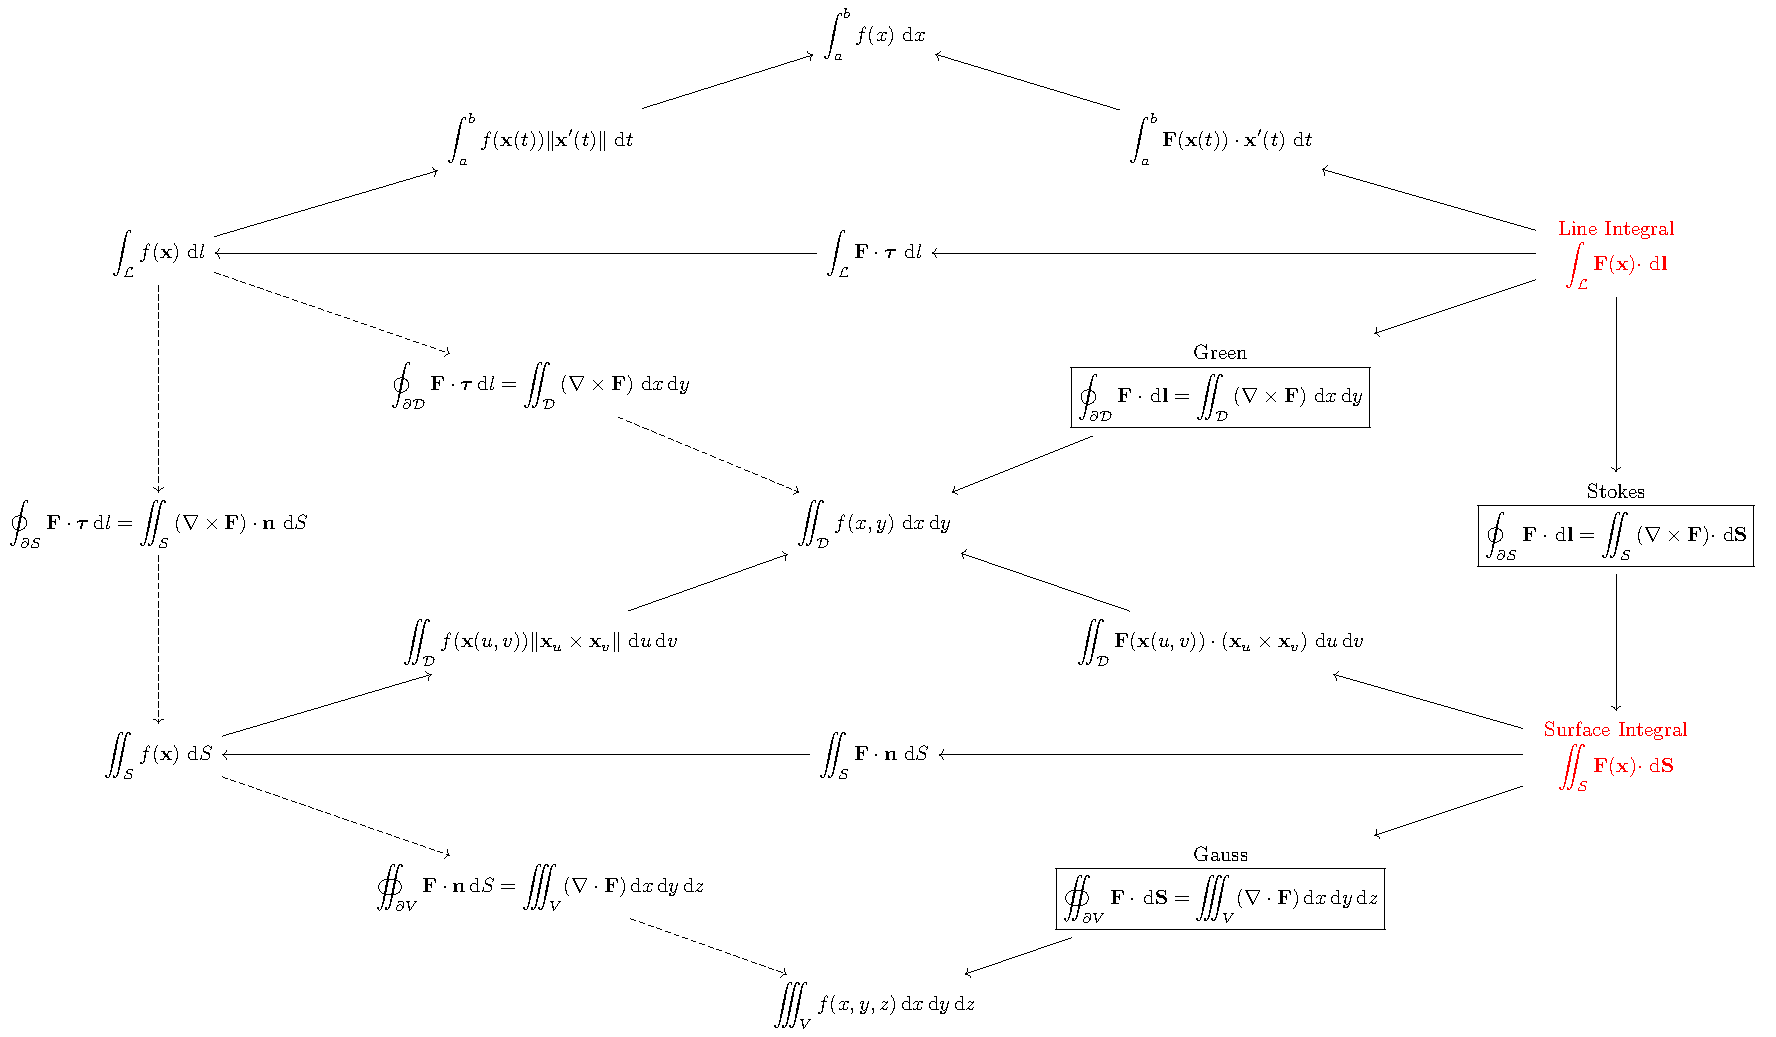
\includegraphics[width=\linewidth]{fig/multivar-integral-relationship.pdf}
\end{figure}
\par 三大公式用外微分形式表示,如$\partial\mD$表示$\mD$区域的边界.
\par 关于第二型线积分和面积分化为定积分或重积分的方法如下
\\
\begin{minipage}[H]{0.5\linewidth}
\[\begin{aligned}
\int_\mL\vF\cdot\diff\vl&=\int_\mL\vF\cdot\vtau\diff l\\
&=\int_a^b\lrp{\vF\cdot\frac{\vx'(t)}{\|\vx'(t)\|}}\|\vx'(t)\|\diff t\\
&=\int_a^b\vF(\vx(t))\cdot\vx'(t)\diff t
\end{aligned}\]
\end{minipage}
\begin{minipage}[H]{0.5\linewidth}
\[\begin{aligned}
\iint_\mS\vF(\vx)\cdot\diff\vS&=\iint_\mD \vF\cdot\vn\diff S\\
&=\iint_\mD \lrp{\vF\cdot\frac{\vx_u\times\vx_v}{\|\vx_u\times\vx_v\|}}\|\vx_u\times\vx_v\|\diff u\diff v\\
&=\iint_\mD \vF(\vx(u,v))\cdot(\vx_u\times\vx_v)\diff u\diff v
\end{aligned}\]
\end{minipage}
\\
\par 因而上述$\vx'(t)$与$\vx_u\times\vx_v$是切向量和法向量,但并\textbf{不是单位}模长(见\ref{sub:sub:sec:tangent}和\ref{sub:sub:sec:normal}节)

\subsection{积分与路径无关}
\begin{theorem}
设$D$为平面单连通区域,函数$P(x,y)$,$Q(x,y)$在$D$上有\textbf{连续偏导数},则下列四个命题等价
\begin{enumerate}
	\item 沿$D$中任一逐段光滑闭曲线$L$,有
	\[\oint_LP\diff x+Q\diff y=0\]
	\item 对$D$中任一逐段光滑曲线$L$,曲线积分
	\[\int_LP\diff x+Q\diff y\]
	与路径无关,只与$L$的起点和终点有关
	\item 微分式$P\diff x+Q\diff y$在$D$内是原函数$u(x,y)$的全微分,即有
	\[\diff u=P\diff x+Q\diff y\]
	\item 在$D$内每一点有
	\[\vmat{\vi&\vj\\\pd{P}{y}&\pd{Q}{x}}=0\]
\end{enumerate}
注意:前面三个结论对复连通区域也等价
\end{theorem}
求原函数通常通过两段折线来求
\[u(x,y)=\int_{x_0}^x P(x,y_0)\diff x+\int_{y_0}^yQ(x_0,y)\diff y+C\]
当然也可以直接凑微分得到,如
\[\begin{aligned}
&\quad(2x\cos y-y^2\sin x)\diff x+(2y\cos x-x^2\sin y)\diff y\\
&=(2x\cos y\diff x-x^2\sin y\diff y)+(2y\cos x\diff y-y^2\sin x\diff x)\\
&=\diff (x^2\cos y)+\diff (y^2\cos x)\\
&=\diff (x^2\cos y + y^2\cos x)
\end{aligned}\]
\begin{theorem}[奇点]
关于奇点(不满足$\pd{Q}{x}=\pd{P}{y}$的点)的结论
\begin{enumerate}
	\item 对$D$内任意一条不包围奇点的闭曲线$L$,有
	\[\oint_LP\diff x+Q\diff y=0\]
	\item 环绕某一奇点的任意两条简单闭曲线$L_1,L_2$的积分相等,即
	\[\oint_{L_1}P\diff x+Q\diff y=\oint_{L_2}P\diff x+Q\diff y\]
	这个公共值称为该奇点的循环常数
	\item 环绕某一奇点$n$圈的光滑闭曲线$L$,其中$n_1$圈为正向,$n_2$圈为负向,$n_1+n_2=n$,则积分
	\[I=\oint_LP\diff x+Q\diff y\]
	等于该点循环常数的$n_1-n_2$倍
	\item 若不自相交光滑闭曲线$L$包围了$k$个奇点,则沿$L$正向的积分
	\[I=\oint_LP\diff x+Q\diff y\]
	等于这$k$个奇点循环常数之和
\end{enumerate}
\end{theorem}
\begin{definition}[原函数]
若$\diff u(x,y)=P(x,y)\diff x+Q(x,y)\diff y$,则称$u(x,y)$为$P\diff x+Q\diff y$的原函数
\end{definition}
\par 注意看积分区域包不包含奇点,若包含则需分类讨论
\begin{example}
设$L$为不经过$(-2,0)$和$(2,0)$点的简单闭曲线,求
\[\begin{aligned}
I&=\oint_L\left[\frac{y}{(x-2)^2+y^2}+\frac{y}{(x+2)^2+y^2}\right]\diff x\\
&+\left[\frac{2-x}{(2-x)^2+y^2}+\frac{-(2+x)}{(x+2)^2+y^2}\right]\diff y
\end{aligned}\]
\end{example}
\begin{analysis}
依题意有
\[\begin{aligned}
P(x,y)&=\frac{y}{(x-2)^2+y^2}+\frac{y}{(x+2)^2+y^2}\\
Q(x,y)&=\frac{2-x}{(2-x)^2+y^2}+\frac{-(2+x)}{(x+2)^2+y^2}
\end{aligned}\]
可求得$A(-2,0),B(2,0)$为奇点,当$(x,y)\ne A,B$时$\pd{P}{y}=\pd{Q}{x}$.
设$L$包含的区域为$D$
\begin{enumerate}
	\item 若$D$不包含$A,B$,则由格林公式
	\[I=\iint_D\lrp{\pd{Q}{x}-\pd{P}{y}}=0\]
	\item 若$D$包含$A$和$B$,则分别以$A,B$为圆心,以很小的正数$\eps$为半径作圆$r_1,r_2$,使得$r_1,r_2\in D$且$r_1\cap r_2=\varnothing$,有积分等于奇点循环常数之和,即
	\[I=\oint_{r_1}P\diff x+Q\diff y+\oint_{r_2}P\diff x+Q\diff y\]
	设
	\[\begin{aligned}
	P_1&=\frac{y}{(x-2)^2+y^2}\qquad&Q_1&=\frac{2-x}{(2-x)^2+y^2}\\
	P_2&=\frac{y}{(x+2)^2+y^2}\qquad&Q_2&=\frac{-(2+x)}{(x+2)^2+y^2}
	\end{aligned}\]
	在$r_1$包围的区域$D_1$内,$P_1,Q_1$均有连续偏导数,且$\pd{P_1}{y}=\pd{Q_1}{x}$;\\
	在$r_2$包围的区域$D_2$内,$P_2,Q_2$均有连续偏导数,且$\pd{P_2}{y}=\pd{Q_2}{x}$;
	故有
	\[\begin{aligned}
	I&=\oint_{r_1}P_2\diff x+Q_2\diff y+\oint_{r_2} P_1\diff x+Q_1\diff y\\
	&=\frac{1}{\eps^2}\oint_{r_1}y\diff x-(2+x)\diff y+\frac{1}{\eps^2}\oint_{r_2}y\diff x+(2-x)\diff y\\
	&=\frac{1}{\eps^2}\iint_{D_1}(-2)\diff x\diff y+\frac{1}{\eps^2}\iint_{D_2}(-2)\diff x\diff y\qquad\mbox{格林公式}\\
	&=-4\pi
	\end{aligned}\]
	\item 若$D$只含$A,B$中其中一个,同上理可得$I=-2\pi$
\end{enumerate}
综上,
\[I=\begin{cases}0&\text{$D$不含$A,B$}\\-2\pi&\text{$D$中只含$A,B$中任一个}\\-4\pi&\text{$D$包含$A,B$}\end{cases}\]
\end{analysis}